\section{Datacrawler}
\label{Datacrawler}
The main goal of the datacrawler is to deliver the required datasets as specified in chapter \ref{datasets}. The input to the datacrawler is simply a domain, which is provided by the ground truth. Depending on the configuration the output of the datacrawler can vary from a single screenshot (\ref{DatasetVersion1}) to a complete graph of the given domain (\ref{DatasetVersion2}).

The following section (\ref{datacrawler_requirements}) will profoundly discuss the requirements in functionality for the datacrawler, which will serve as a basis for discussion for the decision between the frameworks \texttt{Puppeeter} and \texttt{Chromium Embedded Framework} (\ref{datacrawler_framework_language}). Afterwards we will give an overview of the architecture (\ref{datacrawler_architecture}) and highlight the idea of \textit{DataModules} in the crawler (\ref{datacrawler_datamodulesystem}). Following that, we will discuss profoundly all developed \textit{DataModules} with their role in the datacrawler (\ref{datacrawler_screenshot_datamodule}, \ref{datacrawler_mobilescreenshot_datamodule}, \ref{datacrawler_url_datamodule}). We will wrap up the internals of the datacrawler by taking a look into the workflow of the datacrawler (\ref{datacrawler_workflow}).

In the last section (\ref{datacrawler_scale}) we will discuss how we successfully designed a sophisticated system to scale-out the datacrawler reducing the total dataset creation time on Google Cloud Platform.  

\subsection{Requirements}
\label{datacrawler_requirements}
The requirements in functionality for the datacrawler arise from the dataset specifications (\ref{DatasetVersion1}, \ref{DatasetVersion2}). The next section will derive the requirements from the dataset specifications and discuss them profoundly.

\subsubsection{Browser Emulation}
\label{browser_emulation}
One of the major requirements for the datacrawler is to find a convenient way of emulating a web browser. According to the dataset specifications, for every given website a screenshot $\tensorsym{I}$ has to be taken. In addition to that, every screenshot must represent the website as the user would see in a common browser. The latter and other attributes such as the loading time $l$ of a website like in a common browser make the emulation of a browser an inevitable requirement. 

\subsubsection{Information Accessibility}
\label{information_accessibility}
Accessing \textit{low-level} information such as the \textit{HTTP-Request} to change the \textit{user-agent} to generate a mobile screenshot $\tensorsym{M}$ (\ref{datacrawler_mobilescreenshot_datamodule}) or the \textit{Document Object Model (DOM)} (\ref{datacrawler_url_datamodule}) to generate edges $a$ in the graph according to dataset version 2 specification (\ref{DatasetVersion2}) is inevitable. The datacrawler has to be able to manipulate internal data structures and even able to inject own \textit{JavaScript-code} (\ref{datacrawler_screenshot_datamodule}) on the website.

\subsubsection{Modularity}
\label{modularity}
The datacrawler has to be as modular for allowing us to extend the datacrawler easily and decide which attribute should be calculated. This requirement in flexibility is raised from the fact that our dataset specifications might change over the time or new ones might be added.

This flexibility led to a sophisticated architecture such as the \text{DataModule-System} (\ref{datacrawler_datamodulesystem}), which makes it possible to pass the dataset specification directly into the datacrawler.

\subsubsection{Scalability}
\label{scalability}
Both dataset versions require the analysis of at least 100,000 websites. Therefore, datacrawler has to be horizontally scalable to allow the analysis of multiple domains at once, and efficient in terms analysis time and start-up time. An inefficient and not scalable datacrawler would lead to multiple days of required analysis time and reflect also in high infrastructure costs.

\subsection{Framework}
\label{datacrawler_framework_language}
The previous section has shown some of the intricate requirements for the datacrawler. To answer those requirements in the given time frame, we investigated in frameworks, which would do most of the heavy-lifting for us such as networking, I/O or rendering of the website.

In our research we focused on the evaluation of frameworks, which base on the most common browser \texttt{Google Chrome} \cite{CommonBrowsers}. This section will introduce two frameworks \texttt{Puppeteer} and \texttt{Chromium Embedded Framework} (\texttt{CEF}), compare both and discuss our decision for \texttt{CEF}. Both frameworks are providing an API to instrument the well-known browser \texttt{Chrome}.

\subsubsection{Puppeteer}
\texttt{Puppeteer} is a open-source library for the JavaScript runtime \texttt{Node.js}, which provides a high-level API to control instances of the browsers \texttt{Chrome} or \texttt{Chromium}. One of the main goals of \texttt{Puppeteer} is to grow adoption in automated browser testing \cite{PuppeteerFAQ}.  For this purpose, it wraps the \texttt{Chrome DevTools Protocol} in JavaScript, which allows web developers to instrument, inspect and debug instances of \texttt{Chrome}. Technically, the protocol is HTTP-based and exposed as a RESTful API at the port for debugging by \texttt{Chrome}.

The protocol offers a varies number of functionalities, which are grouped into domains \cite{DevToolsProtocol}. Some of the interesting domains for our use-case are:
\begin{description}
	\item[Page]: API to load and take a screenshot of the given website.
	\item[DOM]: API to read and manipulate the DOM of the given website.
	\item[Network]: API to intercept network requests, track downloaded data and network issues.
	\item[Emulation]: API to emulate different geolocation, network bandwith and mobile devices.
\end{description}

During start up \texttt{Puppeteer} starts an instance of \texttt{Chrome}, attaches to the instances using the port for debugging and afterwards custom code of the user will be executed against the instance. The instance will be started in \texttt{headless}-mode meaning that no UI will be visible.

\texttt{Puppeteer} fulfills all requirements (\ref{datacrawler_requirements}) raised from the dataset specifications:
The requirement of \textbf{Browser Emulation} (\ref{browser_emulation}), since it is using an instance of \texttt{Chrome} to render websites. The requirement of \textbf{Information Accessibility} (\ref{information_accessibility}), due to functionalities in the domains DOM and Network. Furthermore \textbf{Modularity} (\ref{modularity}) is given per se by using JavaScript as the programming language, which makes the use of polymorphism possible as used in DataModule-System (\ref{datacrawler_datamodulesystem}). The usage of \texttt{Chrome} ensures efficiency in terms of loading, rendering websites and retrieval of website information. Moreover, the combination of \texttt{Chrome} and \texttt{Puppeteer} can be scaled-out easily fulfilling the last requirement \textbf{Scalability} (\ref{scalability}) by using our system described in \ref{datacrawler_scale}.

\subsubsection{Chromium Embedded Framework}
\texttt{Chromium Embedded Framework (CEF)} is an open-source framework for embedding the \texttt{Chromium} browser into other applications. The main goal of \texttt{CEF} is to enable developers in adding web browsing functionality such as using HTML, CSS and JavaScript to create application UI. Well-known applications such as \texttt{Adobe Acrobat}, \texttt{Spotify Desktop} and \texttt{MATLAB} are using \texttt{CEF}.

\texttt{CEF} was designed ground-up with performance and ease-use in mind. The framework exposes \texttt{C++} interfaces with default implementation for all features requiring little or no integration work. Furthermore, the community added wrappers for the base implementation to support a wide-range of operating systems and programming languages.

\texttt{CEF} has in total three versions, whereas \texttt{CEF 2} was abandoned due to the appearance of the \texttt{Chromium Content API} which will be discussed later. \texttt{CEF 1} is a single process implementation and based on the old \texttt{Chromium WebKit API}, due to deprecation of the \texttt{Chromium WebKit API} it is no longer supported and developed. \texttt{CEF 3} is a multi process implementation and based on the current \texttt{Chromium Content API}.

As the \texttt{Chromium} code base has grown, it was inevitable to avoid opaque dependencies and features in the wrong places. Therefore the \textit{content module} was introduced, which contains the core functionality of \texttt{Chromium}. The \texttt{Chromium Content API} wraps the \texttt{content module} and offers isolation for developers from the core functionalities \cite{ChromiumContentAPI}.
\texttt{CEF 3} insulates the user from the underlying complexity of \texttt{Chromium} by using the \texttt{Chromium Content API} and offering production-quality stable APIs \cite{CEFGeneralUsage}. The offered and consumed APIs as well as the multi-process architecture will be profoundly discussed in \textbf{Datacrawler Architecture} (\ref{datacrawler_architecture}).

Through the use of \texttt{Chromium Content API}, \texttt{CEF 3} provides a close integration between the browser and the host application including support for custom JavaScript objects and JavaScript extensions. Moreover, the host application is able to control resource loading, intercept the network, navigation and many more, while taking advantage of the same performance and technologies available in the \texttt{Google Chrome Web browser} \cite{CEFGeneralUsage}.

\texttt{CEF 3} clearly fulfills the requirement of \textbf{Browser Emulation} (\ref{browser_emulation}) and \textbf{Information Accessibility} (\ref{information_accessibility}). Moreover, \textbf{Modularity} (\ref{modularity}) and \textbf{Scalability} (\ref{scalability}) is also given by using \texttt{C++} and the core functionalities of \texttt{Chromium}.

\subsubsection{Framework Decision}
Both \texttt{Puppeteer} and \texttt{CEF} fulfill the requirements raised by the dataset specifications. At first glance it seemed a free choice, but after close investigation we found additional points speaking for \texttt{CEF}. In the end we decided to use \texttt{CEF 3} for the datacrawler, due to following additional points:
\begin{itemize}
\item Our team has an outstanding expertise in \texttt{C++}, which is the programming language used in both \texttt{CEF 3} and \texttt{Chromium}.
\item While as \texttt{Puppeteer} is limited to the \texttt{Chrome DevTools Protocol}, \texttt{CEF 3} provides low-level access to the core of \texttt{Chromium}. This ultimately gives us more freedom of control.
\item \texttt{CEF 3} is integrated into \texttt{Chromium} leading to a faster start-up and execution time Whereas \texttt{Puppeteer} has to start up an instance of \texttt{Chrome} and communicate via a RESTful HTTP API, which represents an addition overhead.
\end{itemize}
\subsection{Datacrawler Architecture}
\label{datacrawler_architecture}
One of the major points in the design and implementation of the Datacrawler was to meet the \textbf{Modularity} requirement (\ref{modularity}). This led to the development of the sophisticated \textit{DataModule}-System and introduced the concept of \textit{Datamodules}. The Datamodule-System represents the architecture of the Datacrawler. 

Before diving into our implementation details by introducing the \textit{DataModule}-System, we will discuss how applications using \texttt{CEF 3} are build and work in general (\ref{datacrawler_cef_architecture}). Following that, we will introduce the \textit{DataModule}-System (\ref{datacrawler_datamodulesystem}) in great detail giving the required information to understand how \textit{Datamodules} work. Afterwards we will discuss how we take a screenshot of a website and tackle the challenge of detecting when a website has finished loading in the \textit{Screenshot}-Datamodule (\ref{datacrawler_screenshot_datamodule}). Beyond that we will discuss how we take screenshots by emulating a mobile device (\ref{datacrawler_mobilescreenshot_datamodule}) and collect URLs by traversing the DOM (\ref{datacrawler_url_datamodule}). In the end we will show how we generate and output the graph (\ref{datacrawler_graph}) and wrap up by taking a look into the end-to-end workflow of the Datacrawler (\ref{datacrawler_workflow}). 

\subsubsection{CEF 3 Application Structure}
\label{datacrawler_cef_architecture}
\texttt{CEF 3} is based on multiple processes. It can mainly be divided into the \textit{browser}-process and \textit{render}-process.

\begin{itemize}
\item The browser-process represents the host process of the application, which handles window creation, painting and network access. Furthermore, most of the application logic will run in the browser-process. 
\item Multiple render-processes are responsible for rendering websites, executing JavaScript and running some application logic. Following the process model of \texttt{Chrome}, \texttt{CEF 3} spawns for every unique origin a render-process ensuring resource isolation, parallelism and better failure management.
\end{itemize}

The separate spawned processes communicate using \textit{Inter-Process Communication} (IPC). Application logic implemented in browser- and render-process can communicate by sending asynchronous messages as \textbf{URL-Datamodule} (\ref{datacrawler_url_datamodule})  will show. Other processes are spawned when needed such as the \textit{plugin}-process for handling of plugins like \textit{Flash}.

In general \texttt{CEF 3} application consists of the class \texttt{CefApp} and \texttt{CefClient}. \texttt{CefApp} is responsible for process-specific callbacks such as returning handler for a custom render-process implementation (\ref{datacrawler_url_datamodule}). Whereas \texttt{CefClient} is responsible for handling browser-instance-specific callbacks such as returning handler for a customer website render implementation (\ref{datacrawler_screenshot_datamodule}). It contains most of the application logic and is being used to create browser instances. As mentioned before, it can be used to control the browser-instance with custom implementation.

The following will briefly describe the start-up of an application using \texttt{CEF 3}:
\begin{enumerate}
	\item The \texttt{CefExecuteProcess}-method is used with custom implementation of \texttt{CefApp} to start separate processes. The application executable will be started multiple times representing new processes.
	\item \texttt{CreateBrowser} is used with custom implementation of \texttt{CefClient} to create a browser-instance. The browser instance is created in the browser-process, which means that there is only one browser at a time. Futhermore, an initial URL is passed to the browser-instance.
	\item In the implementation of \texttt{CefClient} \texttt{CefMessageLoop}-method is executed, which starts the event loop of the browser-instance. This means that browser-instance will start loading the given URL, handling network, rendering and many more. \texttt{CEF} takes care of spawning and using of existing render-processes.
	\item Once \texttt{CefQuitMessageLoop}-method is called, the message loop will be quit.
\end{enumerate}

\subsubsection{DataModule-System}
\label{datacrawler_datamodulesystem}
The naming of the DataModule-System derives from the purpose to bind, execute instances of Datamodules, collect results and output the dataset. The system consists of several components, which enable developers to implement and execute Datamodules independently increasing flexibility and reducing potential failures. In a plugin-and-play-manner developers can easily develop and add Datamodules to the Datacrawler.

The main idea of a Datamodule is to represents a single attribute in the dataset, which is calculated and added independently from other attributes to the dataset. In addition, each Datamodule can be individually configured and turned on or off by the user.

 We are heavily utilizing polymorphism language feature of \texttt{C++} to enable previous mentioned features. Thus, a Datamodule consists of the implementation of the following interfaces:

\begin{itemize}
	\item[\texttt{DataModuleBaseConfiguration}] This interface has to be implemented by each Datamodule. It is responsible for the creation and configuration of instances of a given Datamodule.
	\item[\texttt{DataModuleBase}] The DatamoduleBase-interface represents the core of each Datamodule. Most of application logic of the Datamodule will be implemented here.
	\item[\texttt{DataBase}] This has to be implemented if the result of the Datamodule should be stored in the graph. It represents the results of the implemented Datamodule.
\end{itemize}

Figure \ref{datacrawler_uml_diagram} represents a simplified UML-Diagram of the Datacrawler with the most important classes, interfaces and methods for understandig the DataModule-system. The figure does not show the implementation details of \texttt{CEF 3}, which are isolated and located in each Datamodule.

The class \texttt{Datacrawler} represents the entrypoint of the Datacrawler. It holds an instance of the class \texttt{DatacrawlerConfiguration}, which is responsible to load the user-defined Datamodules configuration using the method \texttt{loadConfigFromJSON()}. Upon successful loading, the Datacrawler creates instances of Datamodules using the method \texttt{createInstance()}. The interface method is implemented individually by each Datamodule reflecting custom Datamodule configuration. 

Once the \texttt{process(url)}-method has been called with an URL in \texttt{Datacrawler}, we create \texttt{NodeElement} representing the starting node and add it into our graph. Our graph is implemented as a key-value list, whereas the key represents the URL and the value our \texttt{NodeElement}-object. For dataset version 1 (\ref{DatasetVersion1}) we assume to have a single node with a single screenshot. Afterwards we go through the our instantiated Datamodules and execute custom implementation of the method \texttt{process(url)}. At this point an isolated browser instance is created using \texttt{CEF 3}, which executes Datamodule-specific browser implementation. As soon as a Datamodule returns, we add the results to the current \texttt{NodeElement} and add \texttt{NodeElement} to our graph. 

Upon the completion of all Datamodules for a given URL, we add all generated edges of the Datamodule \texttt{URLDatamodule} into a FIFO queue in \texttt{Datacrawler}. In section \ref{datacrawler_url_datamodule} we will discuss how and which URLs we select as edges of a node. Afterwards we repeat the process of creating a new object of \texttt{NodeElement}, executing of Datamodules, adding the results into new \texttt{NodeElement} and URLs to our FIFO queue for the oldest entry. We skip a given URL if there is a key-value pair in our list or if we reach our maximal number of nodes in the graph. \improve{Discuss number of max nodes}

\begin{figure}
	\centering
	\includegraphics[scale=0.35]{resources/breadth-first}
	\caption{This figure illustrates the breadth-first search. The numbers in the nodes show the order in which nodes are expanded in breadth-first search. It shows that all nodes reachable from a selected nodes are expanded, before selecting the first node encountered and expanding the nodes reachable from it. E.g the selected node is \textbf{1} and the nodes \textbf{2}, \textbf{3} \textbf{4} are expanded, before we select \textbf{2} and expand the node \textbf{5} and \textbf{6}.}
	\label{datacrawler_breadth_search}
\end{figure}

The use of the FIFO queue leads to breadth-first search in our graph in opposition to a deep search, which is implemented using a LIFO queue. The breadth-first search means that we expand all nodes reachable from the edges of our current node and selecting the oldest entry as new node, rather than using the first edge, expanding the reachable node and selecting it as the current node. By using the breadth-first search, we maximize the number of directly reachable nodes from a given node. This leads to a wide and dense rather than deep and sparse graph. \improve{Discuss why we need a dense graph rather than a sparse} Figure \ref{datacrawler_breadth_search} illustrates the breadth search exemplary.

\begin{figure}
	\centering
	 \includegraphics[scale=0.65]{resources/datacrawler_uml_diagram}
	 \caption{The figure shows the simplified UML-diagram of the datacrawler with the most important classes and methods. Classes in the white boxes represent essential components of the DataModule-System such as the classes \texttt{Datacrawler}, \texttt{DatacrawlerConfiguration}, \texttt{NodeElement} and the interfaces \texttt{DataModuleBaseConfiguration}, \texttt{DataModulBase} and \texttt{DataBase}. Classes in the red boxes represent implementation of DataModules such as the \texttt{URLDatamodule} (\ref{datacrawler_url_datamodule}), \texttt{ScreenshotDatamodule} (\ref{datacrawler_screenshot_datamodule}) and \texttt{MobileScreenshotDatamodule} (\ref{datacrawler_mobilescreenshot_datamodule}).}
	\label{datacrawler_uml_diagram}
\end{figure}

\subsubsection{Screenshot-Datamodule}
\label{datacrawler_screenshot_datamodule}
The Screenshot-Datamodule is responsible for visiting a website by a given URL and taking a screenshot upon successful loading as specified in section \ref{DatasetVersion1}. The entrypoint of the Datamodule is \texttt{process(url)}-method in \texttt{ScreenshotDatamodule}-class. Upon completion, the Datamodule returns an instance of \texttt{Screenshot}, which contains a screenshot and information about width and height of the screenshot.

In general the Screenshot-Datamodule addresses three difficult problems with the help of \texttt{CEF 3}: 

\begin{enumerate}
	\item \textbf{Any} website given by URL  has to be loaded without exceptions.
	\item \textbf{Every} website has to be rendered in a format to take a screenshot from.
	\item The Datamodule has to detect when a given website has finished loading to take a screenshot.
\end{enumerate}

The following sections will profoundly discuss how the Screenshot-Datamodule successfully addresses previous mentioned problems with the use of \texttt{CEF 3}.

\paragraph{Loading} 
The Screenshot-Datamodule consists of \texttt{ScreenshotDatamodule} and implementations of the interfaces \texttt{CefClient} and \texttt{CefRenderHandler}. In \texttt{process(url)}-method of \texttt{ScreenshotDatamodule} a synchronous browser instance is created with our implementation of \texttt{CefClient} and the given URL. As mentioned in section \ref{datacrawler_cef_architecture} \texttt{CefClient} is responsible for browser-instance-specific callbacks and hence the place to customize the browser for our needs. Therefore, we implement \texttt{CefClient} and overwrite the method \texttt{GetRenderHandler()} to return a custom implementation of \texttt{CefRenderHandler}. The browser instance will now use our implementation of \texttt{CefRenderHandler} to paint the website during loading.

The use of a synchronous browser instance allows us to iterate through the event loop of the browser instance by ourselves until we take a screenshot of the given website. This is mandatory for both threads, which are created directly after the browser instance and play a critical role in detecting if a website has finished loading. 

\paragraph{Rendering}
In the world of \texttt{Chromium} \textit{rendering} relates to the process of parsing, transforming of website data to generate DOM, executing JavaScript, applying CSS and painting of the website. 

In Screenshot-Datamodule the interface \texttt{CefRenderHandler} is not responsible for rendering a website, but only for the painting to the end user device. In our implementation, we have implemented the \texttt{GetViewRect()} and \texttt{OnPaint()}-method of \texttt{CefRenderHandler}. Latter is the place to paint the website to the end user device, whereas we define in \texttt{GetViewRect()} the height and width of the output from the browser. In case of \texttt{CEF 3} the \texttt{OnPaint()}-method is invoked each time if the browser instance detects invalidation caused by changes in the DOM and CSS. These changes can be caused by a loading website, animations or dynamically changing content due to custom JavaScript code.

In each invocation of \texttt{OnPaint()} following information are passed as parameters:

\begin{itemize}
\item Reference to the current browser instance.
\item Reference to the buffer, where image information are kept about the website.
\item Information about the height and width of the given website.
\end{itemize}

The buffer is an array of respectively one byte encoded single characters, where each character is representing a channel of the color space \texttt{BGRA}. Consequently, a single pixel corresponds to four characters in the buffer. The array represents the pixels from the left most to the right most starting from the top of the viewport in repeating order of the color space. Thus, the buffer itself contains only information about visible area as defined in \texttt{GetViewRect()}, which reflects the viewport of the browser.

On each invocation we allocate total of $4 * \texttt{width} * \texttt{heights}$ bytes in the memory and copy the content of our buffer into it. Once we detect the website has finished loading, we can access the latest painting of \texttt{OnPaint()} from the memory.

\paragraph{Detection}
In our current implementation the browser instance calls \texttt{OnPaint()}-method to update the view port, whenever a change occurs on the website. In practice this means that our implementation might return screenshots of partially loaded websites, if we access to the buffer at a bad time. The simple solution to wait a given time $t$ and take the most recent screenshot is not an option. This static approach would lead to high analysis time per website and violate the scalability requirement (\ref{scalability}). We have to detect, when a given website has finished loading to reduce our analysis time per website.

In general, there are multiple states during the loading of a website, which can be interpreted that a given website has finished loading. Before we discuss our approaches to tackle this complex problem, we define our understanding when a website has finished loading:

\begin{center}
\textit{A website has finished loading, if and only if all elements are painted on the view port and no new elements are being painted.}
\end{center}

Our definition includes the painting and rendering of the given website in the browser and represents the \textit{natural} behavior of a browser. The following definition does not include those aspects:

\begin{center}
\textit{A website has finished loading, if and only if all the content of the website has been downloaded successfully from the internet.}
\end{center}

Based on our assumption we have developed two algorithms for this problem:

\begin{itemize}
	\item Detection based on calculation of \textit{change} matrices. 
	\item Detection based on \texttt{OnLoadingStateChange()}-method of \texttt{CEF 3} and hard coded waiting time.
\end{itemize}

Our algorithm based on calculation of change matrices, assumes that the number of changed pixels per screenshot will dramatically reduce over time. In other words, given the screenshots $I_{t}, I_{t+1}, I_{t+2}\in \{0, ... , 255\}^{width\times height \times 4}$ taken at times $t$, $t+1$,  and $t+2$ respectively, the total number of changed pixels  $|\Delta_{t,t+1}|$ between $I_{t}$ and $I_{t+1}$ will be less than $|\Delta_{t+1,t+2}|$. Furthermore, we assume that the $|\Delta|$ will converge for $t \rightarrow \infty$ meaning that the website has finished loading. The blue line in figure \ref{plot_assumption_number_changes} illustrates our assumption exemplary.

In order to calculate the number of changed pixels between two screenshots $I_{t}$ and $I_{t+1}$, we have introduced the change matrix $C_{t,t+1} \in \{0,1\}^{width\times height}$. Each element $c_{i,j} \in C_{t,t+1}$ represents the change state between the pixels $\mathbf{s}^{t}_{i,j,} \in I_{t}$ and $\mathbf{s}^{t+1}_{i,j,}  \in I_{t+1}$, which in turn are in $\{0, ... , 255\}^{4}$ representing the color space \texttt{BGRA}.

On every invocation of \texttt{OnPaint()} we calculate the change matrix $C_{t,t+1}$ on basis of the current screenshot $I_{t+1}$ and the screenshot $I_{t}$ of the previous invocation. The following applies for each element $c_{i,j} \in C_{t,t+1}$ :

\[
c_{i,j} =
\begin{cases}
1,& \text{if $\mathbf{s}^{t}_{i,j,} \neq \mathbf{s}^{t+1}_{i,j,}$ } \\
0,              & \text{otherwise}
\end{cases}
\]

We compute the total number of changes from $I_{t}$ to $I_{t+1}$ with matrix norm $|| C_{t,t+1}||$ and save it in every invocation of \texttt{OnPaint()} for later use. In addition, we also calculate the maximum number changes per screenshot with $width \times height$ and call it $C_{MAX}$. The red line for \texttt{nationalgeographic.com} in figure \ref{plot_assumption_number_changes} shows that the number of changes is indeed converging, but not stable as expected. We take this into account and calculate on every invocation the average $C_{AVG}$ for the number of changes at $t-n, t-n+1, ..., t$, whereas $n$ is defined in the Datamodule configuration and $t$ represents our current screenshot. Putting everything together we detect if a given domain has finished and take a screenshot by following equation is true:

\[
{\frac{C_{\text{AVG}}}{C_{\text{MAX}}} \leq p_{C}; \quad   {\frac{C_{\text{AVG}}}{C_{\text{MAX}}}}, p_{\text{C}} \in [0,1]}
\]

The fraction ${\frac{C_{\text{AVG}}}{C_{\text{MAX}}}}$ describes the average in percentage of changes over the last $n$ screenshots and $p_{C}$ is the user-defined threshold. 

Furthermore, we have observed that for websites such as \texttt{timodenk.com} the \texttt{OnPaint()}-method is only called for a limited number of times. This might not be enough to leverage our detection algorithm. Therefore we have implemented a thread, which starts upon every \texttt{OnPaint()}-invocation a timer. The timer has the goal to return a screenshot, if \texttt{OnPaint()}-method has not been invoked for the user-defined time.  

\begin{figure}
\centering

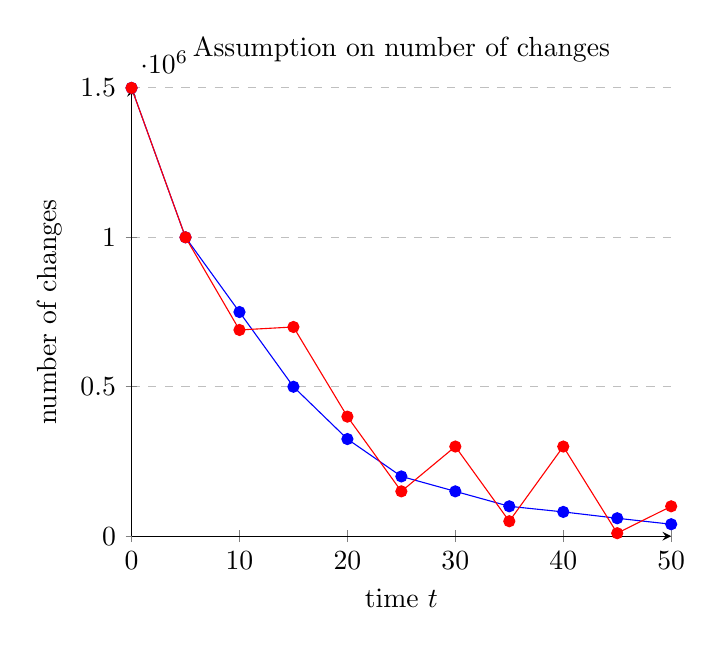
\begin{tikzpicture}
\begin{axis}[
title={Assumption on number of changes},
axis lines = left,
xmin=0, xmax=50,
ymin=0, ymax=1500000,
xlabel = time $t$,
ylabel = {number of changes},
ymajorgrids=true,
grid style=dashed,
]
%Here the blue parabloa is defined
\addplot[
color=blue,
mark=*,
]
coordinates {
	(0,1500000)(5,1000000)(10,750000)(15,500000)(20,325000)(25,200000)(30,150000)(35,100000)(40,81250)(45,60000)(50,40000)
};
\addplot[
color=red,
mark=*,
]
coordinates {
	(0,1500000)(5,1000000)(10,690000)(15,700000)(20,400000)(25,150000)(30,300000)(35,50000)(40,300000)(45,10000)(50,100000)
};
\end{axis}
\end{tikzpicture}
\caption{The figure illustrates exemplary in blue our assumption regarding the number of total changes $|| C_{t,t+1}||$ from $I_{t}$ to $I_{t+1}$. It shows that the number of total changes dramatically reduce and converge for $t \rightarrow \infty$. The red line illustrates the actual measured number of changes for \texttt{nationalgeographic.com} with the resolution $1920$ in width and $1080$ in height. }
\label{plot_assumption_number_changes}
\end{figure}

Our second algorithm implements \texttt{OnLoadingStateChange()}-method of \texttt{CefLoadHandler}, which will be invoked upon a website has been loaded successfully. During invocation the parameter \texttt{isLoading} is passed, which is true if the given website has been loaded and false if not. However, this variable does not indicate that the given website has been painted successfully. It only indicates the browsers is ready to paint the given website. Therefore we have implemented a timer, which will start upon \texttt{isLoading} is true, run for a user-defined time and return the content of the buffer.

In addition both algorithms implement a thread, which starts a timer upon the loading of a website. This timer represents a hard timeout for the Screenshot-Datamodule and will run for a user-defined time. After timeout it will ultimately return a screenshort. Thus, guaranteeing us to return the buffer  in any circumstances.

\begin{table}[]
	\centering
	\begin{tabular}{lllll}
		Algorithm based on & Partially Loaded & Fully Loaded & \% of Partially Loaded  & Total \\ \hline \hline
		change matrices & 13 & 87 & 13 \% & 100 \\ \hline
		\texttt{OnLoadingStateChange()} & 3 &  97 & 3 \% & 100
	\end{tabular}
\caption{The table illustrates the performance of our algorithms based on change matrices and \texttt{OnLoadingStateChange()} for the top 100 websites from \texttt{Open PageRank}. The websites are manually evaluated by us. A website is categorized as partially loaded, if it is obviously missing parts of the website, and fully loaded, if not. The approach using \texttt{OnLoadingStateChange()} performs with $3\%$ of partially loaded websites better than our approach with change matrices with $13\%$. }
\label{table_compare_algorithm_screenshot}
\end{table}

We have manually evaluated both approaches using the top 100 website in \texttt{Open PageRank} (\ref{OpenPageRank}). Our results are described in table \ref{table_compare_algorithm_screenshot}. They show that the algorithm based on \texttt{OnLoadingStateChange()} outperforms the algorithm based on change matrices. This ultimately leads to our decision to use \texttt{OnLoadStateChange()} as our preferred detection algorithm.

\subsubsection{MobileScreenshot-Datamodule}
\label{datacrawler_mobilescreenshot_datamodule}
The MobileScreenshot-Datamodule is responsible for visiting a website by a given URL and taking a screenshot upon successful loading. The \texttt{process(url)}-method is the entrypoint for the Datamodule. In contrast to the Screenshot-Datamodule, the visited website has to be in mobile resolution and mobile view leading to a screenshot taken from a mobile device (\ref{DatasetVersion2}).

In total there are two ways to request a mobile view for a website:

\begin{itemize}
	\item Visit the website with mobile device resolution e.g $375$ in width and $667$ in height
	\item Declare the \textit{user-agent} as a mobile device e.g  \texttt{Mozilla/5.0 (iPhone CPU)}
\end{itemize}

While the resolution represents the size of the view port in which the given website is being displayed, the user-agent represents the identification of the browser. It is a request header containing a characteristic string that allows the communication partner to identify application type, operating system, software vendor and version of the requesting browser instance. The request header is being send on every HTTP method such as \texttt{GET}. The \texttt{CEF 3} uses a desktop user-agent per default as figure \ref{compare_resolution} shows.

Our initial assumption, that requesting a website with mobile resolution would lead to a mobile view, was right for a majority of the websites. But figure \ref{compare_resolution_useragent} shows that there are exceptions such as \texttt{youtube.com}, where it is not enough to scale down the resolution. Hence, we consider in our implementation to use a mobile resolution and user-agent. While we reuse most of the implementation of the Screenshot-Datamodule (\ref{datacrawler_screenshot_datamodule}) such as the loading, rendering and detection, we extend and change the implementation at specific points to support mobile view.

First we adjust the resolution of the browser instance in \texttt{GetViewRect()} to mobile resolution, which is given by the mobile screenshot requirement described in dataset version 2 (\ref{DatasetVersion2}). Second, we intercept all outgoing requests from the browser instance and add the required mobile user-agent header. This is done by providing a custom implementation of the interface \texttt{CefRequestHandler} having the primary goal to handle browser requests. In \texttt{CefRequestHandler} we implement the \texttt{OnBeforeResourceLoad()}, which is invoked every time before a request is send. During invocation the outgoing request \texttt{CefRequest} is passed as parameter, which allows us to modify the request for our needs. The request contains beside the body, target URL, HTTP method also a key-value store representing the header section of the request. Upon every invocation we modify the key-value store and overwrite the key \texttt{User-Agent} with the value \texttt{Mozilla/5.0 (iPhone [...]) Chrome/71 [...] Mobile [...]}. The latter represents the Chrome browser on the mobile device \texttt{Apple iPhone}. 

The interception and modification led us to successfully emulate a mobile device from our Datacrawler, allowing us to take screenshots from a mobile device.

\begin{figure}
	\centering
	\begin{subfigure}{.6\textwidth}
		\centering
		\includegraphics[width=.5\linewidth]{resources/screenshot_resolution}
		\caption{}
		\label{compare_resolution}
	\end{subfigure}%
	\begin{subfigure}{.6\textwidth}
		\centering
		\includegraphics[width=.5\linewidth]{resources/screenshot_resolutionanduseragent}
		\caption{}
		\label{compare_useragent}
	\end{subfigure}
	\caption{This figure shows two screenshots taken from the website \texttt{youtube.com}. The figures (a) and (b) were taken with a browser instance having the resolution $375 \times 667$. In addition, we changed the user-agent of the figure (b) to represent a mobile device and use the default user-agent of \textit{CEF 3}. The usage of the mobile user-agent clearly shows that the website is being displayed for mobile devices in figure (b), whereas in figure (a) not.}
	\label{compare_resolution_useragent}
\end{figure}

\subsubsection{URL-Datamodule}
\label{datacrawler_url_datamodule}
The URL-Datamodule represents one of the most complex Datamodules in the Datacrawler. It is responsible for returning a set of valid URLs for a given website, server and client errors occurred during loading, title, loading time and download size of the website. While calculating and returning so many attributes in a single Datamodule is contrary to the principles of the Datamodule-System (\ref{datacrawler_datamodulesystem}), we had to do the trade-off in order to (1) reduce overall development and (2) analysis time. The latter arises from the fact that for every single attribute we have to create a new browser instance and reload the entire website, which takes a tremendous amount of computing resources and time. Thus, complexity URL-Datamodule arises by calculating multiple attributes at once and the usage of different processes and their communication based on \textit{IPC}.

In general, the URL-Datamodule is executed by invoking the \texttt{process(url)}-method. Upon successful completion it returns an instance of \texttt{URLCollection}, which is added to \texttt{NodeElement} and contains previous mentioned attributes. Similar to other Datamodules, we implement \texttt{CefClient} and other interfaces with our custom implementation and start a browser instance for the given URL. In the following, we will profoundly discuss the implementation by discussing each attribute calculation solely.

\paragraph{URLs}
The URL-Datamodule has to return valid URLs. This attribute is specified as following in the specification of dataset version 2 (\ref{DatasetVersion2}):

\begin{center}
	\textit{Each edge $a$ represents a possible navigation from web page $v_1$ to $v_2$ [...] and has the same Fully Qualified Domain Name.}
\end{center}

According to the specification a given URL is only valid if it is a possible navigation and has the same FQDN. Possible navigation means that only URLs found as a \texttt{href}-attribute in \texttt{<a>}-tags in the \texttt{HTML}-code of the website can be considered as valid. This follows from the fact that in \texttt{HTML} \texttt{<a>}-tag is the only tag, which allows the user to navigate to other pages from the current viewed page. While possible navigation describes where to find valid URLs, equality in FQDN describes which URLs to choose from a set of URLs.
For example the FQDN for the URL \texttt{http://web.samedguener.com/index.html} is \texttt{web.samedguener.com}. While the URL \texttt{http://web.samedguener.com/contact.html} found on the website would be valid with \texttt{web.samedguener.com} as FQDN, \texttt{http://samedguener.com/} would not since \texttt{samedguener.com} is the FQDN.

While it would be possible to access the URLs by downloading the \texttt{HTML}-code of the visited page, it would take a very long time and be tedious work to parse the code and build the DOM to access the URLs. 
\paragraph{Loading Time}

\paragraph{Client and Server Errors}

\paragraph{Title}

\paragraph{Download Size}

\subsubsection{Generating the Graph}
\label{datacrawler_graph}
\subsubsection{Datacrawler Workflow}
\label{datacrawler_workflow}

In general Datacrawler can be divided mainly into three functional parts:

\begin{enumerate}
	\item[Initializiation] : The Datacrawler reads the Datamodule configuration from a local file and initializes the Datamodules accordingly.
	\item[Crawling] : The Datacrawler crawls the passed domain according to the activated Datamodules and calculates attributes for the dataset.
	\item[Output] : The Datacrawler generates and saves the graph to the disk.
\end{enumerate}


\subsection{Scaling the Datacrawler}
\label{datacrawler_scale}

\subsubsection{Requirements}
\label{datacrawler_scale_requirements}

\subsubsection{The Scale Architecture}
\label{datacrawler_scale_architecture}


